\documentclass[10pt,a4paper]{article}
\usepackage[utf8]{inputenc}
\usepackage[T1]{fontenc}
\usepackage{amsmath}
\usepackage{amsfonts}
\usepackage{amssymb}
\usepackage{graphicx}
\usepackage{kotex}
% Package for si units
\usepackage{siunitx}

% Packages for making pictures with LaTeX
\usepackage{tikz}
\usetikzlibrary{shapes,arrows,positioning,fit,backgrounds,calc}
\usepackage{pgfplots}
\pgfplotsset{compat=1.16}

% Package to superimpose text on an image
\usepackage[percent]{overpic}

\begin{document}
	%
	\title{\LaTeX \,\,문서작성법\\
        Figures using for economics\\ 
        TIKZPICTURE, PGFPLOTS \& OVERPIC}
	\maketitle


	\begin{abstract}
	몇개의 샘플을 가지고 작성해 볼 것이다. 일반적인 수요와 공급 법칙 그리고 예산선에 대한 그림을 그려볼 것이다. \texttt{tikz}, \texttt{pgfplots} 벡터를 이용한 그래프를 작성할 수 있다. \texttt{tikz} 와 \texttt{overpic}를 가지고 다른 곳에 적용해볼 수 있다.  
	\end{abstract}
	%
	%
	\vspace{0.5cm}\noindent
	%
	%
	%
	Figure~\ref{fig:analytical}, is the first example illustrating how to graph analytical functions with \texttt{tikzpicture} directly in latex. and how to colourise and label them.
	%	
	\begin{figure}[!ht]
		\centering
		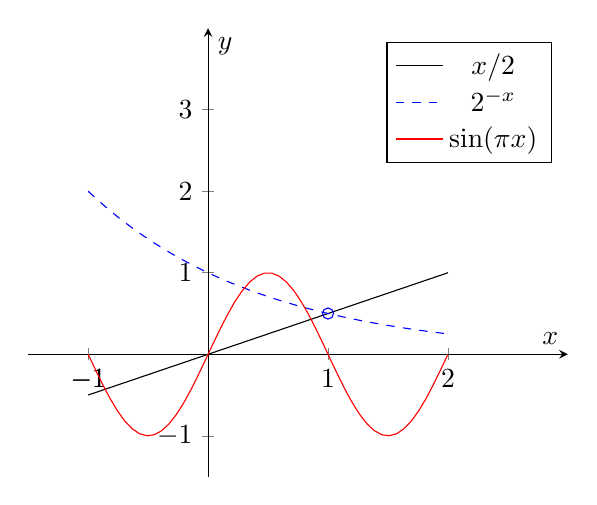
\begin{tikzpicture}
		\begin{axis}
			[
			legend pos= north east,
			axis lines = center,
			domain=-1:2,
			xlabel=$x$,
			xmin=-1.5,
			xmax=3,
			xtick={-1,-1,0,1,2},
			ylabel=$y$,
			ymin=-1.5,
			ymax=4,
			ytick={-1,0,1,2,3},
			samples=50,
			]
			\addplot [] {x/2};
			\addplot [blue,dashed] {2^(-x)};
			\addplot [red] {sin(deg(pi*x))};
			\addplot [blue, mark = o] coordinates {( 1, 1/2)};
			\legend{$x/2$,$2^{-x}$,$\sin(\pi x)$}
		\end{axis}
		\end{tikzpicture}
		\caption{Graphs of three analytical functions.}
		\label{fig:analytical}
	\end{figure}
	%
	
	The second example is illustrated by Fig.~\ref{fig:xf1f2}, which depicts data from the plain-text file \texttt{xf1f2.txt} located in the subfolder \texttt{Data}. The data file has $3$ columns containing in its $1$\textsuperscript{st} column a list of $x$-values and values for the data $y=f_1(x)$ and $f_2(x)$, listed in column $2$ and $3$, respectively.
	%
	\begin{figure}[!ht]
		\centering
		\begin{tikzpicture}
		\begin{axis}[
		xlabel={$x$ (\SI{}{\metre})},
		xmin=2,
		xmax=256,
		xmode=log,
		log basis x={2},
		ylabel={label  (unit)},
		ymin=0.4,
		ymax=1,
		enlargelimits=false,
		legend pos=north east
		]
		\addplot[blue,mark=o] table[x index=0,y index=1] {Data/xf1f2.txt};
		\addplot[red,mark=o,only marks] table[x index=0,y index=2] {Data/xf1f2.txt};
		\legend{$f_1$,$f_2$}
		\end{axis}
		\end{tikzpicture}
		\caption{Graphs of the data in the text file \texttt{xf1f2.txt} for the two functions $y=f_1$ and $f_2$.}
		\label{fig:xf1f2}
	\end{figure}
	%
	
	The second example is a flowchart including images inserted using the package \texttt{overpic}. It illustrates a solution procedure which can be applied to estimate the wear depth according to \eqref{eq:wear_depth_plastic}, i.e.,
	%
	\begin{equation}\label{eq:wear_depth_plastic}
	{\Delta h}_{ij}  = k\Delta sp_{ij} + {u_p}_{ij}.
	\end{equation}
	%
	
	%
	\begin{figure}
		\centering
		\begin{tikzpicture}[
		node distance = 3mm and 9mm,
		block/.style = {rectangle, draw, rounded corners,
			text width =8em},
		blockfig/.style = {text width =10em},
		cloud/.style = {draw, ellipse, aspect=1.2}
		]
		% Place nodes
		
		\node [blockfig] (twosurfini)
		{\begin{overpic}[width=1\textwidth]{Figures/two_surfs_ini.pdf}
			\put (10,33) {$ h_u$}
			\put (10,9) {$ h_l$}
			\end{overpic}};
		\node [block, left= of twosurfini.west] (init) {Initial surface topographies and relative position};
		
		\node [blockfig, below=of twosurfini.south] (twosurfcontact)
		{\begin{overpic}[width=1\textwidth]{Figures/two_surfs_contact.pdf}
			\put (25,33) {$ p$}
			\end{overpic}};
		\node [block, left= of twosurfcontact.west] (cm) {Run enhanced CM solver to compute $p$ \& $u_p$};
		
		\node [blockfig, below=of twosurfcontact.south] (twosurfwear)
		{\begin{overpic}[width=1\textwidth]{Figures/two_surfs_wear.pdf}
			\put (32,19) {$ \Delta h + u_p$}
			\end{overpic}};
		\node [block, left= of twosurfwear.west] (wear) {Compute wear depth using \eqref{eq:wear_depth_plastic}};
		
		\node [blockfig, below=of twosurfwear.south] (twosurfworn)
		{\begin{overpic}[width=1\textwidth]{Figures/two_surfs_worn.pdf}
			\put (23,23) {$h_l - (\Delta h + u_p)$}
			\end{overpic}};
		\node [block, left= of twosurfworn.west] (worn) {Remove material from the softer surface};
		
		\node [blockfig, below=of twosurfworn.south] (twosurfshift)
		{\begin{overpic}[width=1\textwidth]{Figures/two_surfs_shift.pdf}
			\put (45,25) {$\Delta s$}
			\end{overpic}};
		\node [block, left= of twosurfshift.west] (shift) {Update relative position by $\Delta s$};
		
		% Draw connections
		\draw[-latex'] (init.south) -- (cm.north);
		\draw[-latex'] (cm.south) -- (wear.north);
		\draw[-latex'] (wear.south) -- (worn.north);
		\draw[-latex'] (worn.south) -- (shift.north);
		
		\node [coordinate, left = 1cm of shift] (shiftcr) {}; %% Coordinate on the right of shift
		\node [coordinate, left = 1cm of cm] (cmcr) {}; %% Coordinate on the right of cm
		\draw[-] (shift.west) -- (shiftcr);
		\draw[-] (shiftcr) -- (cmcr);
		\draw[-latex'] (cmcr) -- (cm.west);
		
		\end{tikzpicture}
		\caption{\small Flow chart of the solution procedure used for wear prediction. It shows how to combine \texttt{tikz} and \texttt{overpic} to overlay/embed intrinsic latex text onto images created elsewhere}
		\label{fig:flowchartwear}
	\end{figure}
	%
이 예제들은 꽤나 한줄 씩 치면서 연습하기 좋을 것이다. 이 수업에서 대체적으로 다룰 것은 latex으로 tkiz 패키지를 사용하여 그리거나 연도별 데이터 혹은 상품들의 집합 등을 표현 할 table들과 fig 들을 작성할것이고 , 이후에 작성될 fig중에서는 일반적인 수요 공급 곡선들에 대한 논의들이 있다. 2차원 공간상의 형태로 

 \section{실습 예제 1번}
아래는 그래프를 그리기 위한 패키지에 대해서 설명하면서 overleaf에서 그 

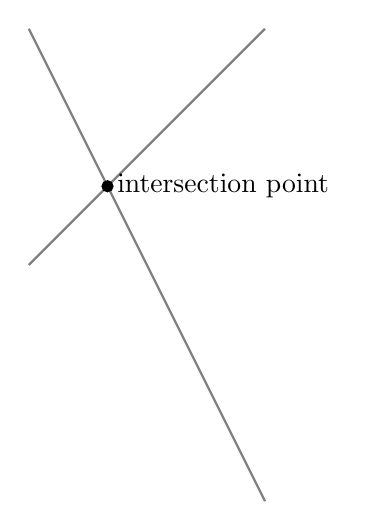
\begin{tikzpicture}
    \draw[gray, thick] (-1,2) -- (2,-4);
    \draw[gray, thick] (-1,-1) -- (2,2);
    \filldraw[black] (0,0) circle (2pt) node[anchor=west]{intersection point};
\end{tikzpicture}

 working with the basic elements, points and lines 

 \begin{tikzpicture}
     \draw (-2,0) -- (2,0);
     \filldraw[gray] (0,0) circle(2pt);
     \draw (-2,-2) .. controls(0,0) .. (2,-2);
     \draw (-2,2) .. controls (-1,0) and (1,0) .. (2,2);
     
 \end{tikzpicture}

the  start point and endpoint 

\begin{tikzpicture}[domain=0:5,scale=1,thick]
\usetikzlibrary{calc}   %allows coordinate calculations.
 
%Define linear parameters for supply and demand
\def\dint{4.5}          %Y-intercept for DEMAND.
\def\dslp{-0.5}         %Slope for DEMAND.
\def\sint{1.2}          %Y-intercept for SUPPLY.
\def\sslp{0.8}          %Slope for SUPPLY.
 
\def\pfc{2.5}           %Price floor or ceiling
 
\def\demand{\x,{\dslp*\x+\dint}}
\def\supply{\x,{\sslp*\x+\sint}}
 
% Define coordinates.
    \coordinate (ints) at ({(\sint-\dint)/(\dslp-\sslp)},{(\sint-\dint)/(\dslp-\sslp)*\sslp+\sint});
    \coordinate (ep) at  (0,{(\sint-\dint)/(\dslp-\sslp)*\sslp+\sint});
    \coordinate (eq) at  ({(\sint-\dint)/(\dslp-\sslp)},0);
    \coordinate (dint) at (0,{\dint});
    \coordinate (sint) at (0,{\sint});
    \coordinate (pfq) at  ({(\pfc-\dint)/(\dslp)},0);
    \coordinate (pfp) at  ({(\pfc-\dint)/(\dslp)},{\pfc});
    \coordinate (sfq) at  ({(\pfc-\sint)/(\sslp)},0);
    \coordinate (sfp) at  ({(\pfc-\sint)/(\sslp)},{\pfc});
 
% DEMAND
    \draw[thick,color=blue] plot (\demand) node[right] {$P(q) = -\frac{1}{2}q+\frac{9}{2}$};
    
% SUPPLY
    \draw[thick,color=purple] plot (\supply) node[right] {Supply};
 
% Draw axes, and dotted equilibrium lines.
    \draw[->] (0,0) -- (6.2,0) node[right] {$Q$};
    \draw[->] (0,0) -- (0,6.2) node[above] {$P$};
        
    %Price floor and ceiling lines
    \draw[dashed,color=black] plot (\x,{\pfc}) node[right] {$P_c$};
    \draw[dashed] (pfp) -- (pfq) node[below] {$Q_d$};
    \draw[dashed] (sfp) -- (sfq) node[below] {$Q_s$};
     
\draw[->,baseline=5] ($(0,{\pfc})+(-1.5,0.7)$) node[label= left:Price Ceiling] {} -- ($(0,{\pfc})+(-.1,0.1)$);
 
\end{tikzpicture}
\end{document}